\documentclass{tufte-handout}
\usepackage{amsmath,amsthm}

\usepackage{pgfplots}
\pgfplotsset{width=\textwidth}

\newtheorem{claim}{Claim}[section]
\title{\sf Exact Algorithm for Independent Set}
\author{}

\newcommand{\mis}{\textsc{MIS}}
\newcommand{\nodeu}{\ensuremath{\tiny u}}
\newcommand{\nodev}{\ensuremath{\tiny v}}

\tikzset{
  auto,node distance=5mm,thick,
  remaining node/.style={thick,circle,draw,minimum size=3mm,fill=black!10},
  remaining edge/.style={thick},
  mis node/.style={dotted,circle,draw,minimum size=3mm,fill=blue!20},
  removed node/.style={dotted,circle,draw,minimum size=3mm},
  removed edge/.style={thin,dotted}
}

\begin{document}
\maketitle

\section{Independent Set Lab Report}
by Erik Westrup and Dmitry Basavin

\subsection{Correctness}
Algorithm R1 correctly computes $\alpha(G)$ because $[\ldots]$.

\noindent
Algorithm R2 correctly computes $\alpha(G)$ because $[\ldots]$.

\subsection{Empirical Running time}

\paragraph{Experiments.}

\medskip
\noindent
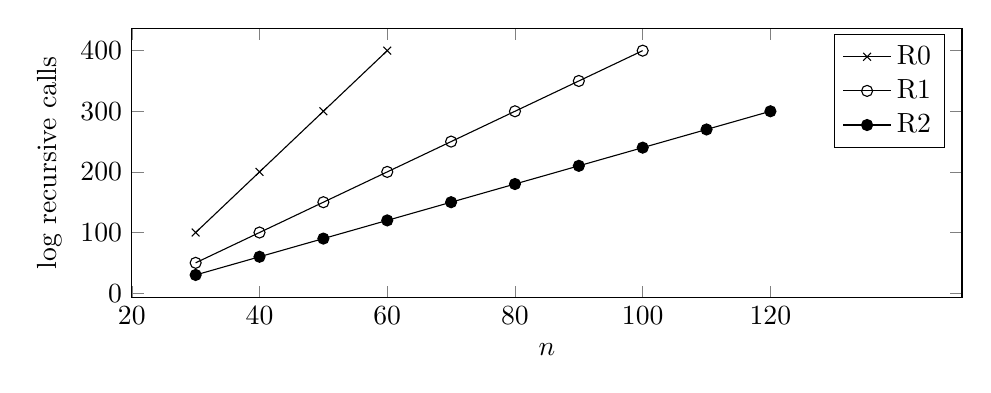
\begin{tikzpicture}
\begin{axis}[
  height= 5cm,
  xlabel=$n$,
  ylabel={log recursive calls},
  xmin = 20,  xmax = 150,
  xtick =       {20,40,60,80,100,120},
  xticklabels = { $20$, $40$, $60$, $80$, $100$, $120$},
  x tick label as interval = false,
  scaled ticks = false
]
    \addplot[color=black, mark=x] 
	coordinates {
	(30, 100)
	(40, 200)
	(50, 300)
	(60, 400)
    };
    \addlegendentry{R0}

    \addplot[color=black, mark=o] 
	coordinates {
	(30, 50)
	(40, 100)
	(50, 150)
	(60, 200)
	(70, 250)
	(80, 300)
	(90, 350)
	(100, 400)
    };
    \addlegendentry{R1}

    \addplot[color=black, mark=*] 
	coordinates {
	(30, 30)
	(40, 60)
	(50, 90)
	(60, 120)
	(70, 150)
	(80, 180)
	(90, 210)
	(100, 240)
	(110, 270)
	(120, 300)
    };
    \addlegendentry{R2}
\end{axis}
\end{tikzpicture}

The running times of algorithm~$R_0$, $R_1$, and $R_2$ appear to be
$[\ldots],[\ldots],$ and $[\ldots]$, respectively..

\subsection{Theoretical Upper Bound}

Denote be $T_i(n)$ the worst runtime of algorithm Ri on \emph{any} graph on $n$ vertices.
Note that $T_i(n)$ is a non-decreasing function of $n$.
For $R_0$ we can conclude that
\begin{align*}
T_0(n) &\leq\max(T_0(n-1), T_0(n-1)+T_0(n-1-d_{\mbox{max}})) \\ &\leq T_0(n-1)+T_0(n-2)
\end{align*}
with $d_{\mbox{max}}$ the degree of the vertex we branch on. The hard part is the one when there are no isolated vertices, in which case the vertex $u$ we are branching on has at least one neighbor. 

For R1 we have that
 \[
 T_1(n)=[\ldots]
 \]

For R2 we have that
 \[
 T_2(n)=[\ldots]
 \]
\paragraph{Worst Case Upper Bound}
The running times of algorithm~$R_0$, $R_1$, and $R_2$ are in
$[\ldots],[\ldots],$ and $[\ldots]$, respectively. \newpage

\section{Optional}
Add more ``algorithmic intelligence'' to the algorithm $R_2$ in order to tackle the instance in data/g130.in.
Try to make it run in less than 10,000,000 recursive calls. 

Suggestions for possible speed-ups:
\begin{itemize}
\item Is there some clever (branching) rule for vertices of degree 3?
\item Can we use the information of the largest found independent set so far, to reduce further computation time?
\item What if the graph gets disconnected?
\end{itemize}


\end{document}
